\section{Economic properties}

\subsection{Emission Rules}

Ergo emission will last for 2080799 blocks (8 years with a 2 minute block interval) --- for the
first 525600 blocks (2 years) 75 Erg will be issued per block and after that the block reward will be
reduced by 3 Erg every 64800 blocks (3 months).
To fund the development, during the first 655200 blocks (2.5 years), the part of the block reward that
exceeds 67.5 will go to a treasury instead of a miner.  (see Fig.~\ref{fig:emission}).

\begin{figure}[H]
    \centering
    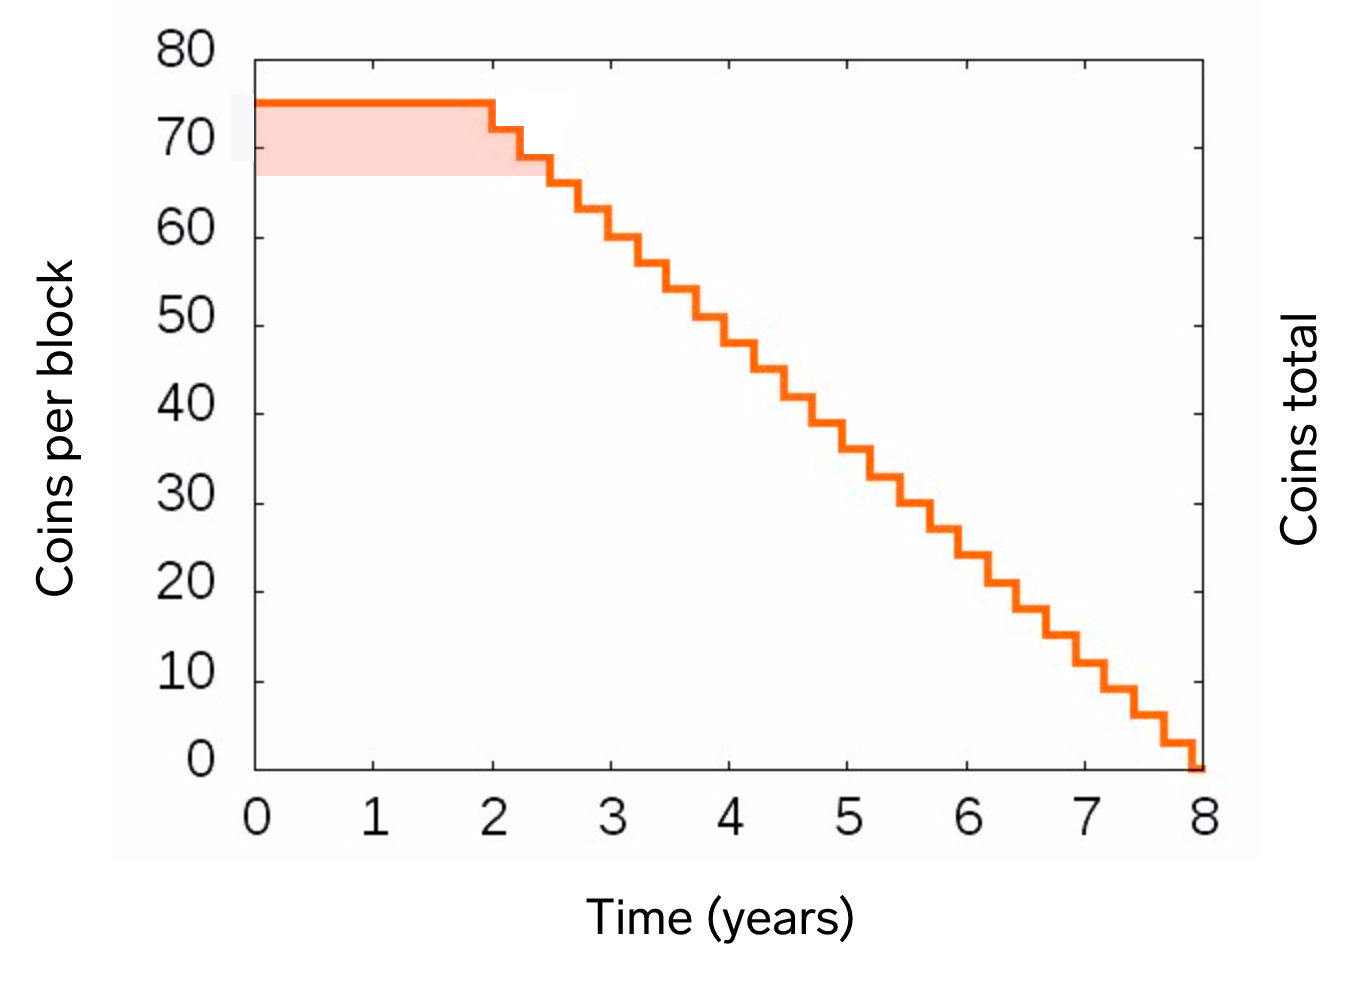
\includegraphics[width=\textwidth]{img/emission.jpg}
    \caption{Ergo emission rule
    \label{fig:emission}}
\end{figure}


Instead of having an implicit emission rule via a special type of transaction (e.g. coinbase transaction in Bitcoin),
Ergo coins emission rule is defined explicitly by sigma-state transactional language.

Miners reward of 93409132.5 Erg will be created in the genesis state in a box,
protected by the script, defined at https://git.io/fhgOq.
This script allows a miner to take only a part of all coins every block.
Transaction that spends this output should have exactly 2 outputs: the first one should
have the same protecting script and contain all input coins minus current block reward,
while the second one may be collected by the current block miner after at least
720 blocks delay.

Treasury part emission will be kept in the genesis state in a box with 4330791.5 Erg and
will be protected protected by the script, defined at https://git.io/fhg3q.
First output of the transaction that spends this box should at least have the value of the
remaining treasury.
In addition, conditions from R4 register of this box should be satisfied,
allowing to protect this output from undesirable spent.
At the beginning R4 register will contain 2-of-3
multisignature proposition with the hardcoded public keys.

Ergo emission will start from zero with no pre-mine. As proof-of-no-pre-mine genesis state
will contain an additional box with 1 Erg inside protected by unspendable proposition.
This box registers R4-R6 will contain latest news headlines from the Guardian, Xinhua and Vedomosti,
while registers R7-R8 will contain latest block id's from Bitcoin and Ethereum.

\subsection{Demurrage component}

We outline following two properties required for long-term survivability of the chain:

\begin{itemize}
    \item{} coins protected by keys being lost should be returned into circulation.
    Otherwise, after the end of the emission period, amount of the coins
    in the circulation will always decrease and eventually reach zero.
    \item{} nothing should be kept in the state forever and for free.
    Otherwise, the size of the state is always increasing with time, thus reducing clients performance.
\end{itemize}

To achieve this, we propose the following storage fee consensus rules.
Register $R3$ of a box contains tuple $(creation\_height, tx\_id || out\_num)$, where $creation\_height$ provided by a user
is used to determine the block height at the moment of transaction generation.
Transaction can only be put in the block of height $h$ if for every created box its $creation\_height \le h$.

Once the subsidized period for the box ends (that is,
$current\_block\_height \ge box.creation\_height + SP$, see $SP$ value below), anyone~(presumably, a miner) can
create a new box $out$ with the exactly the same content (including the guarding
script) except the monetary value and $R3$ contents. The monetary value is to
reduced by $K \cdot B$ maximum, where $B$ is the spent box~($self$)
size and $K$ is the storage cost for the period $SP$. Thus, the difference is to be paid to the miner.
If box value is less that the storage fee, all the box content including tokens could be spent by the miner.

For efficient lookup~(to find a proper output regarding an expired input without an iteration over transaction outputs),
we require a spending proof for an expired box to be just a context extension which contains only an index of an
output which is trying to spend the box. The variable identifier for the index in the extension is $127$.

We propose the following concrete parameters:
\begin{itemize}
    \item{} $SP$ - length of a period for which box can be stored in a State for free untouched.
    It is a constant, namely, $SP = 1051200 \approx 4$ years.
    \item{} $K$ - cost of storage of 1 byte of data in a State for the period of $SP$ blocks.
    Should be determined by miner votes, $1250000 (nanoErg/SP)$ by default, max value is $2500000$.
\end{itemize}

\knote{Provide a script}
